\chapter{Distributed Algorithms}
% \todo{This chapter is a work in progress.}
Many thanks to the Decentralized thoughts blog.
\section{Models}
Distributed systems and their behaviour and algorithms are designed around the model 
they are expected to work in. The model defines the assumptions and constraints of the system.
For instance, the model may define the network the system is expected to 
work in or faults the servers might encounter.

\subsection{Network Model}

When we discuss Network models, we mainly refer to three types of networks:

\begin{defn}[Synchronous]
    There exists some known and finite time bound $\Delta$.
For any message sent, the adversary can delay its delivery by at most $\Delta$.
\end{defn}

At first thought, the Synchronous model may seem to be good enough. 
Why not just assume, for example, that any message sent over the internet will be delivered by say
 $2$ minutes? First, there is a trade-off:
\begin{itemize}
    \item Setting a large and conservative $\Delta$ of say $10$ minutes may
    indeed always faithfully model the real world.
    However, protocol designers who depend on $\Delta$ may incur very long timeouts and 
    hence degrade performance.
    \item The synchronous model is not realistic.
    In the real world, messages can be delayed by an arbitrary amount of time.
\end{itemize}


\begin{defn}[Asynchronous]
    For any message sent, the adversary can delay its delivery 
    by any finite amount of time.
    In other words, messages can be scrambled and delivered in any order. 
    Furthermore, while a message is delayed 
    by an infinite amount of time, it must eventually be delivered.        
\end{defn}


Unlike the synchrony model, 
the asynchronous model forces protocol designers to assume nothing about network delays.
The outcome is often very robust protocols:

\begin{itemize}
    \item Since they do not depend on any time bound, message delays 
    cannot cause unexpected safety violations.
    \item Since they cannot use any fixed values for timeouts, 
    they must inherently adapt to the actual latency of the system
\end{itemize}

The main problem with the asynchronous model is that protocols in this model tend to be more
complex and harder to reason about. 
Moreover, there are many known complexity gaps between synchrony and asynchrony. Two examples:

\begin{itemize}
    \item The Fischer, Lynch and Paterson \cite[FLP, 1985]{flp} lower bound says 
    that in the asynchronous model, any protocol that solves consensus 
    withstanding an adversary (who can fail-stop just one party) must have an infinite execution.
    \item Authenticated Byzantine Agreement (important problem we will see later\todo{Add reference later}) is possible for 
    $n>2\cdot f$ parties in the synchronous model, but impossible for $n \le3\cdot n$ in the asynchronous model.
\end{itemize}




\emph{Partial synchronous} attempts to capture the best of both worlds.
Informally, in the Partial synchrony model, the system behaves asynchronously 
up to some time called $GST$ (global stabilization time), and after that time it'll behave synchronously.
\emph{Note} that the adversary can delay the $GST$ event by any finite amount
of time and that no protocol can explicitly detect that $GST$ has occurred.
Furthermore, there is no external signal that tells you that $GST$ happened

\begin{defn}[Partially Synchronous \cite{partial-async}]
    There exists some known finite time bound $\Delta$,
    and a special event called GST (global stabilization time) such that:
    \begin{itemize}
        \item The adversary must cause the GST event to happen after 
        some unknown finite time.
        \item Any message that is sent at time $x$ must be delivered by 
        time $\Delta+\max\left(x,GST\right)$.
    \end{itemize}
\end{defn}

Partial synchrony captures the intuition that we would like to design protocols for 
systems that are usually synchronous but have reasonable guarantees, 
even if the synchrony assumptions become temporarily violated by some extreme event
(like a denial of service attack). In particular, a recurring theme in the Partial
synchrony model is to design protocols that are always safe (even when the system
is asynchronous) but provide liveness and termination guarantees only
after GST (only when the system is synchronous).


\begin{xca}[quiz 1.A]
    In the Synchronous model with parameter $\Delta$ which of the following are true:
    \begin{enumerate}
        \item Some message is sent at time $t$ and arrives at time $t+\Delta/4$.
        \item Some message is sent at time $t$ and arrives at time $t+3\Delta$.
        \item Any message sent at any time $t$ arrives at time at most $2t$.
        \item The protocol designer does not know the value of $\Delta$.
    \end{enumerate}


\paragraph{Solution}
        \begin{enumerate}
            \item correct since $t+ \Delta/4$ is less than $t+ \Delta$ which is
            the latest a message sent at time $t$ can arrive.
            \item is false because the adversary can delay the message by at most $\Delta$.
            \item is false because $2\cdot t$ can be greater than $\Delta$.
            \item The protocol designer should set the value of $\Delta$.
        \end{enumerate}

\end{xca}

\begin{xca}[Quiz 1.B]
    In the Asynchronous model which of the following are true:
    \begin{enumerate}
        \item There is some finite number $\Delta$ such that for every finite execution, all
         message delays in that execution are at most $\Delta$.
        \item Some messages that are sent may never arrive to their destinations.
        \item For every finite execution, there is some finite number $\Delta$ such that 
        all message delays in that execution are at most $\Delta$.
        \item The protocol designer can always assume that message sent will arrive after at most one day.
    \end{enumerate}
    \paragraph{Solution}
    \begin{enumerate}
        \item False by definition.
        \item False, all messages arrive, although at an unknown time.
        \item \todo{Verify with Teach} False, the adversary can delay any message by a finite 
        amount of time. Therefore, it can delay the message beyond the execution time.
        % $\forall finite RUNS \exists \Delta $ such that the delay is less than $\Delta$.
        % since Delta is finite, can't the adversary choose $\Delta +1$?
        \item False, the protocol designer cannot assume any time bound.
    \end{enumerate}
\end{xca}


\begin{xca}[Quiz 1.C]
    In the Partially Synchronous model with parameter $\Delta$ which of the following are true:
    \begin{enumerate}
        \item The protocol designer can design protocols that wait till they 
        see the GST event and then take advantage of synchrony.
        \item A message sent $2\Delta$ time before GST will have a delay of at most $3\Delta$.
        \item There is some finite number $\Lambda$ such that for every
         execution, messages sent before GST have a delay of at most $\Lambda$.
         \item A message sent $2\Delta$ time after GST will have a delay of at most $2\Delta$.
    \end{enumerate}
    
    \paragraph{Solution}
    \begin{enumerate}
        \item No. The GST cannot be signaled or detected.
        \item Yes,from the definition. any message sent at time $x$ ($=2\cdot \Delta$) must be delivered by
         time $\Delta + \max(x, GST)$. 
         Consequently, a message sent at time $GST - 2\Delta$ will be delivered at most by time $GST + \Delta$.
        \item no. but if GST is the same for all executions yes, setting $\Lambda$ equal to $GST + \Delta$ implies 
        that every message transmitted before $GST$ will reach its intended recipients by the time $\Lambda$ elapses.
        \item False. it'll have a delay of at most $\Delta$.
    \end{enumerate}
\end{xca}


\begin{xca}[Quiz 1.D]
    Which are true?
    \begin{enumerate}
        \item Any execution in the Partially Synchronous model with parameter
         $\Delta$ is also a legal execution in the Synchronous model with parameter $\Delta$.

        \item Any execution in the Synchronous model with parameter 
        $2 \Delta$ is also a legal execution in the Partial Synchronous model with parameter $\Delta$.

        \item Any execution in the Partially Synchronous model with parameter 
        $2\Delta$ is also a legal execution in the Asynchronous model.

        \item There exists a number $\Delta$, such that any execution in the Asynchronous 
        is also a legal execution in the Synchronous model with parameter $\Delta$.
    \end{enumerate}
    
    \paragraph{Solution}
    \todo{Ask Teach}
    \begin{enumerate}
        \item Yes, by setting $GST=0$, the Partially Synchronous model becomes the Synchronous model.

        \item No, if $GST > 2\Delta$, then the message will be
        delayed beyond the Synchronous model's $\Delta$, which breaks the assumptions.

        \item Yes. Partial async models assume that GST time is unknown and cannot count on it, just like 
        message delays in the Asynchronous model.

        \item No, the statementr $\exists \Delta$ such that $\forall$ async executation is also a legal sync execution,
        is false since we first set the sync model's $\Delta$ and then the async model's $\Delta$.
        since the async model can delay any message by any finite amount of time, it can delay the message beyond the sync model's $\Delta$.

    \end{enumerate}
\end{xca}



\section{Threshold Adversary}
In addition to restricting the adversary's capabilities through a communication model,
 we also require a mechanism to limit the adversary's influence over corrupt parties.

If the adversary has no limits to its power, then there is very little we can do.
Let's begin with the traditional notion of a \emph{threshold adversary} as used in Distributed 
Computing and Cryptography to limit the power of the adversary.


\paragraph{threshold Adversaries}
    Given some $n$ nodes, the adversary controls some $f$ nodes, where $f<n$.
    There are three main types of threshold adversaries:
\begin{enumerate}
    \item \emph{Dishonest majority} $f<n$, the adversary can control all but one. can be called \emph{anytrust} too.
    \item \emph{dishonest minority} $2\cdot f<n$, the adversary controls a minority of nodes (less than half).
    \item $3\cdot f < n$, where the adversary controls less than a third of the nodes.
\end{enumerate}

\subsection{Quorum intersection}
Since the adversary can corrupt $f$ parties, and often this corruption may include crash failures,
 protocols often collect $n-f$ messages to ensure they don't get stuck.
  These sets of $n-f$ parties possess very useful properties based on quorum intersection
   (similar to the Pigeonhole principle).
   Let us describe a few of these:

\begin{thm}[Quorum Intersection 1]
    if $2f<n$, any set of size $n-f$  will have at least one party in their
    intersection.
\end{thm} 
 \begin{proof}
    $2f<n \iff n-2f>0 \iff n-2f +(n-n) >0 \iff n-2f+n>n \iff 2(n-f)>n$
    That is, having two groups of size $(n-f)$ means we have more elements than the entire group.
    So let us denote these sets as $A,B$ (w.l.o.g), and use the 
    inclusion-exclusion principle:
    $|A\bigcap B| = |A| + |B| - |A\bigcup B| = n-f + n-f - n = 2n - 2f - n = n - 2f > 0$.
    as wanted.
 \end{proof}

\begin{thm}[Quorum Intersection 2]
    Given $3f<n$, any set of size $n-f$ will have at least one non faulty party in their intersection.
\end{thm}
proof is similar to the first theorem.

\begin{corollary}[Quorum Intersection 3]
    \todo{add proof.}
    the intesection of two such sets will have at least $f+1$ non faulty parties.
\end{corollary}
As one can notice, $f+1$ means at least one honest between the two sets.
\begin{xca}[Quiz 1.E]
    Which of the following are true:
    \begin{enumerate}
        \item In the dishonest minority model the adversary can corrupt at most half the parties but
         no more than that.
        \item If the adversary can corrupt at most $f<n/3$ parties then for a fixed $f$, the 
        smallest number $n$ where this holds is $n=3f+1$.
        \item If the adversary can corrupt at most $f<n/2$ parties, then any set of $k<n/2$ must 
        contain at least one non-corrupt party.
        \item When $f<n/4$ then any two sets of size $n-f$ have at least $2f$ 
        non-corrupt parties in the intersection.
    \end{enumerate}
    
    \paragraph{Solution}

    \begin{enumerate}
        \item I think so? i mean $n \ge 2f+1$, so the adversary can have one less then half.
        \item Yes.
        \item No, a set of size n/2-1 can contain just honest members.
        \item No, for instance $n=4f+1$, the intersection of these two sets is at most of size $2f+1$ which means we can have 
        $f$ corrupts there, thus we can assume only$f+1$ honests.
    \end{enumerate}


\end{xca}

\begin{xca}[Quiz 1.F]
    Which of the following are true:
    \begin{enumerate}
        \item If $f<n/3$ then any two sets of size $n-f$ intersect with at least $f+1$ non-faulty parties.
        \item If $f<n/5$ then any two sets of size $n-f$ intersect with at least $3f+1$ parties.
        \item If $f<n/4$ then any two sets of size $n-f$ have at least $2f+1$ parties in their intersection.
        \item If $f<n/2$ then any two set of size $n-f$ have at least two parties in their intersection.    
    \end{enumerate}

    \paragraph{Solution}
    \begin{enumerate}
        \item No. interact with f+1 parties. so at least one honest, but not necessarily more.
        \item Yes.
        \item yes.
        \item No.
    \end{enumerate}
\end{xca}

\subsection{proof of work and proof of stake}
both of these don't assume threshold on the number of adversdaries, but on some resoucre (e.g., computation, coins etc).
\todo{sum more from the blog post }
\section{Power of the adversary}
After we fix the communication model, synchrony, asynchrony, or partial synchrony, 
and a threshold adversary we still have 5 important modeling decisions about the adversary power:
\begin{enumerate}
    \item The type of corruption (passive, crash, omission, or Byzantine).
    \item The computational power of the adversary (unbounded, computational, or fine-grained).
    \item The adaptivity of the adversary (static, delayed adaptive, weak adaptive, adaptive, or strongly adaptive).
    \item The visibility of the adversary (full information or private channel).
    \item The mobility of the adversary (fixed or mobile).
\end{enumerate}


\subsection{type of currption}
We have generally treat four types of corruptions:
\begin{description}
    \item[Passive] Also known as Honest-but-curious.
    Will follow the protocol in earnest, but allows the adversary to learn any information in its view.
    \item[Crash] In addition to passive, Once corrupted, the adversary can cause a crash event, which 
    means the party will stop sending or receiving messages (unrecoverable crash).
    \item[Omission] Does not deviate from the protocol, 
    but will lose or wont send messages according to the adversaries will (maliciously).
    \item[Byzantine] in addition to Omission this gives the adversary full power to control the party and take any
     (arbitrary) action on the corrupted party (e.g., send corrupt messages, lie etc).
\end{description}

\emph{Note} that each corruption type subsumes the previous one.


There are more types of failures, but these are the main ones.

\subsection{Computational power}

\begin{description}
    \item[Unbounded] the adversary has unbounded computational power. 
    This model often leads to notions of perfect security or statistical security
    (protocols designed for this model are secure forever).

    \item[Computationally-bounded] the adversary has a polynomial advantage in computational power 
    over the honest parties. 
    Typically, this means that the adversary cannot (except with negligible probability) break the 
    cryptographic primitives being used. 
    For example, typically assume the adversary cannot forge signatures of parties not in its 
    control. All of modern cryptography depends on this type of adversary and typically 
    there is a security parameter that needs to be updated over time (as computation becomes cheaper)
    \item[Fine-grained] there is some concrete measure of computational power and the adversary is 
    limited concretely. This model is used in proof-of-work based protocols
\end{description}


\subsection{Adaptivity}

Adaptivity is the ability of the adversary to corrupt dynamically based on 
information the adversary learns during the execution. \todo{is the adversary still limited to $f$?}

\todo{Edit}
\begin{description}
    \item[static] the adversary has to decide which $f$ parties to corrupt in advance
     before the execution of the protocol. 
     Note that this is always sufficient when the protocol is deterministic because 
     there are no surprises for the adversary. One natural thing for randomized 
     protocols in this setting it to operate on a random subcommittee. This often leads to $O(n)$ message complexity.

    \item[Delayed adaptive] given a parameter $k$, once the adversary asks to corrupt a party,
     the party is corrupted after $k\Delta$ time. 
     Leader based protocols in synchrony and partial synchrony can often obtain $O(1)$ expected time in
     this paradigm (using a weak leader election). 
     Linear-per-view protocols can obtain $O(n)$ expected messages after GST in this model.

    \item[Weak adaptive] 
    Once the adversary asks to corrupt a party, the party is corrupted after 
    it completes sending all its outgoing messages. 
    So while the adversary is adaptive, the actual corruption may be delayed to after the party sends all its messages in 
    that round (or in asynchrony after is sends all the messages it wants to immediately send).
    Sometimes in this model, it is also required that honest parties can safely erase some information 
    in order to get forward security, or assume that messages always maintain FIFO order in each channel.

    \item[Adaptive] Once the adversary asks to corrupt a party,
     the party is immediately corrupted. 
     Messages sent from the party before corruption cannot be erased (so will eventually arrive in 
     asynchrony or in arrive in at most $\Delta$ time in synchrony).

     \item[Strongly adaptive] once the adversary asks to corrupt a party, 
     the party is immediately corrupted. 
     Moreover, messages sent from the party before corruption that have not yet arrived can be erased 
     (or claw-backed) by the adversary. 
     \todo{what?}Some lower bounds assume this model to obtain a constant error. 
\end{description}

\subsection{Visibility}
The visibility is the power of the adversary to see the messages and the states of corrupted and non-corrupted parties.

\begin{description}
    \item[Full information] The adversary sees the internal state of all parties and the content of all
    message sent. 
    This often severely limits the protocol designer. 
    See for example: Feige's selection protocols, or Ben-Or et al's Byzantine agreement.
    Often, the only thing that the adversary cannot do is predict the value of coins that have not been tossed yet.
    
    \item[Private channel] 
    In this model, we assume the adversary cannot see the internal state of honest 
    parties and cannot see the internal content of messages between honest parties. 
    Each time a message between two honest parties is sent, the adversary learns the 
    source, target, and message size. 
    Depending on the communication model, it can decide to delay it by any value that is 
    allowed by the communication model. The adversary can see the full 
    internal state of corrupted parties.

    \item[Oblivious] The adversary can see the header of each message (source, destination, and message 
    length) sent to and from a corrupt party, and based on that can decide its actions 
    (crash, omit, delay, modify) depending on the adversary corruption type and network model. 
    This type of adversary can model an adversary that has peripheral control 
    (via a corrupt NIC, or local router/gateway). 
    An oblivious omission adversary is often used to model an adversary that can maliciously 
    corrupt parties that have a Trusted Execution Enclaves that cannot be corrupted.
\end{description}


For models that are round-based, another visibility distinction is the 
adversary's ability to rush. When does the adversary see the messages sent to 
parties it controls? In the rushing adversary model, the adversary is allowed to see 
all the messages sent to parties it controls in round $i$ before it needs to decide what messages 
to send in its round $i$ messages. In the non-rushing adversary model, the adversary 
must commit to the round $i$ messages it sends before it receives any round $i$ messages from non-faulty parties.

\subsection{Mobility}
In the traditional fixed model the adversary is allowed to corrupt honest parties with 
some fixed budget of up to $f$ parties, but is not allowed to un-corrupt (or heal) 
corrupt parties back to being honest. 
In the mobile model the adversary is allowed to dynamically decide to 
corrupt and un-corrupt parties. 
The total number of corrupted parties at any given time is at most $f$, 
but over time the set of corrupted parties may change. 
It is often required that there is a gap between the time the adversary un-corrupts one party and 
the time it is allowed to corrupt another. 
This model was introduced by Ostrovsky and Yung and exemplified by proactive secret sharing. 
Another modeling decision is whether the party is aware that it is un-corrupted (in which case it may 
be able to remove in-memory corrupt data).




\begin{xca}[Quiz 1.G]
    Against a deterministic protocol:
    \begin{itemize} 
        \item An adaptive adversary has the same power as a static adversary.
        \item A strongly adaptive adversary for omission faults can create executions 
        that an adaptive adversary for omission cannot create.
        \item The full information adversary has more information than the private channel adversary.
        \item The mobile adversary has the same power as a fixed model adversary.
\end{itemize}
    
\paragraph{Solution}
\begin{itemize}
    \item Depends. If the the input is known in advance- it doesn't matter.
    if the input isn't know in advance, then once it is revealed the adversary can take hold of its specific targets.
    Which the static one cannot.

    \item This is not clear enough. does it take time for the adversary to understand whether it wants to corrupt? 
    Can the advesary understand what the participant can send before it does? does it know the input for the system 
    in advance?
    \item Yep, it knows the secret keys of the honest parties too, and can read the messages even before encryption for instance
    \item Not necessarily, it can learn the secrets of the honest parties due time. where the fixed one cannot.
\end{itemize}
\end{xca}



\begin{xca}[Quiz 1.H]
    Which of the following are true:
    \begin{itemize} 
\item Any adversary that can cause $f$ omission corruptions can simulate an adversary that
 can cause $f$ crash corruptions.
\item  Any adversary that can cause $f$ crash corruptions can simulate an adversary that 
can cause $f$ malicious corruptions.
\item  A static malicious adversary can always simulate an adaptive 
adversary that just does crash corruptions (for the same number of corruptions).
\item  An omission corruption adversary can either block incoming message or outgoing messages but not both.
    \end{itemize}
    
\paragraph{Solution}
\begin{itemize}
    \item Yes.
    \item No? we didn't define malicious corruptions, but i assume you mean byzantine?
    \item I don't know, the adversary in adaptive can gain more than f?\todo{NOTE: adversary can at most have f.} 
    \item (no) It can do both.
\end{itemize}
\end{xca}


\begin{xca}[Quiz 1.I]
    Say the first round a protocol chooses a uniformly random sub-committee of 
    size $<f$. Then only parties in the sub-committee send messages for two rounds.
    \begin{itemize} 
        \item A static adversary can always manage to block the sub-committee from sending messages.
        \item A strongly adaptive adversary can always manage to block the sub-committee from sending messages.
        \item A weakly adaptive adversary with parameter $k=3$ can always manage to block the sub-committee from sending messages their second round of messages.
        \item A delayed adaptive adversary can always block the sub-committee from sending messages their first round of messages.
    \end{itemize}
    
\paragraph{Solution}
\begin{itemize}
    \item No, if the subcommittee is chosen by random, then the adversary can't know in advance who to block.
    \item Seems true, it can choose who to corupt after the subcommittee is chosen, and do so immediately.
    \item I don't know what $k=3$ means for weakly adaptive adversary. but it should be able to corrupt by the second round.
    ( it'll learn who is in the comittee by the end of first round and will be allowed to corrupt after everyone sends their messages in that round).
    \item no. it can take X time to block them, which might be too late.
\end{itemize}
\end{xca}

\section{Consensus}
\todo{fill this section from 

https://decentralizedthoughts.github.io/2019-10-15-consensus-for-state-machine-replication/}
\section{Consensus for State Machine Replication}

Let's start with the definition of a state machine.
A state machine, at any point, stores a state of the system.
It receives inputs (also referred to as commands). 
The state machine applies these inputs in a sequential order using a deterministic
transition function to generate an output and an updated state.
A succinct description of the state machine is as follows

\label{smrdef}
  \begin{lstlisting}[language=Python,
    caption={fft algorithm in python}
  ]
state = init
log = []
while true:
  on receiving cmd:
    log.append(cmd)
    state, output = apply(cmd, state)
\end{lstlisting}

Here, the state machine is initialized to an initial state $init$.
When it receives an input $cmd$, it first adds the input to a $log$. 
It then executes the $cmd$ by applying the transition function apply to the state. As a result, it obtains an updated state and an output output.

In a client-server setting, the server maintains the state machine,
 and clients send commands to the server. 
 The output is then sent back to the client.

An example state machine is the Bitcoin ledger. 
The state consists of the set of public keys along with the associated 
Bitcoins (see UTXO \todo{add url}). 
Each input (or cmd) to the state machine is a transaction 
(see \todo{add Bitcoin core api url}).
The log corresponds to the Bitcoin ledger. 
The transition function apply is the function that determines whether a 
transaction is valid, and if it is, 
performs the desired bitcoin script operation (see \todo{add url to script}).

\subsection{Multi-shot consensus - Server Centric Definition}
The central building block of state machine replication is multi-shot consensus.
In this variant of the consensus problem, a set of servers (also called replicas)
 agree on a dynamically growing log of commands.
 These commands arrive as input to the servers over time 
 (presumably from clients but we abstract that away).

Let $\log_i[s]$ be the $s$-th entry in the log of replica $i$. 
Initially, $\log_i[s]=\bot$ for all $s$ and $i$. 
Replica $i$ writes each $\log_i[s]$ only once to a value that is not 
$\bot$.

\paragraph{Requirements}
We demand that the following properties hold:
\begin{description}
    \item[Safety] Non-faulty replicas agree on 
    each log entry, i.e., if two non-faulty replicas $i$ and $j$ have 
    $\log_i[s] \ne\bot$ and $\log_j[s]\ne\bot$ then $\log_i[s] = \log_j[s]$.

    \item[Liveness] Every input $x$ that arrives at 
    a non-faulty replica is eventually recorded in the log,
     i.e., eventually $\exists s$ and non-faulty replica $i$ such that $\log_i[s]=x$.

    \item[Validity] There is an \emph{injective} mapping from the set of 
    log entries (not including $\bot$) to the set of inputs.
    In other words, every log entry must originate from an input and 
    every input appears in the log at most once. 
    Many systems have additional external validity requirements (discussed soon).

    \item[Prefix completeness]
    If a non-faulty replica $i$ has $\log_i[s] \ne\bot$,
    then for all non-faulty replica $j$ and all indices $s'\le s$,
    eventually $\log_j[s'] \ne\bot$ .

\end{description}


\paragraph{Comparison to single-shot consensus, broadcast, and other notes}
The requirements are similar in multi-shot consensus and 
single-shot consensus. However, there are some differences
\begin{description}
    \item[Consensus on a sequence of values] Conceptually, one can sequentially
    compose single-shot consensus instances to obtain multi-shot consensus.
    There are better alternatives, though.

    \item[External validity] Usually multi-shot concensus adds more constraints 
    (depending on the application) to the validity requirement. 
    For instance, all accepted values must be valid transactions.
\end{description}


\todo{insert primary-backup for crash-failure in sync model.}

\begin{xca}[Quiz 1.J]
    Consider a primary backup protocol:
    \begin{itemize} 
        \item Show a concrete execution where the client library gets the same output sent to it more than once.
        \item Show a concrete execution where the backup gets the same command sent to it more than once.
    \end{itemize}

    \paragraph{Solution}
    \begin{itemize}
        \item client sends to primary. primary fails after responding to client, once backup changes view it sends output again.
        \item in the multiple backups case: assume primary is $replica_0$
         client sends command to $replica_0$. 
         it sends to $replica_1$ and $replica_2$ then fails.
         after no heartbeat arrives $replica_1$ resends the last command to $replica_2$. 
         Since $replica_2$ already saw the command - it sees the same command more than once (as wanted).
    \end{itemize}
\end{xca}

\section{Linearization in Distributed Systems}
Multiple nodes accessing replicated data.
How do we define "concistency" in such a system?
This definition should be supported both in terms of concurency, and in terms of failures.

The strongest option is Linearization.
Informally every operation takes effect \emph{atomically}
sometime after it started and before it finished.

So all operations (reads or writes) behave as if executed on a single copy of
the data, managed by a single server (even if there are in fact multiple replicas).
As a result, in a linearized system, every operation always response 
with and "up to date" value ("Strong consistency" is a synonym for linearization).

This is relevant for concurency on a threaded system too.

\emph{Linearziability $neq$ serializability}


Under Linearziability, if operations overlap in real time 
it is valid if the actual (set/get) operations are ordered one or the other.
That is, in linearization the operation must take affect somewhere between
its start and end time.
 
 \begin{figure}[t]
        \centering
        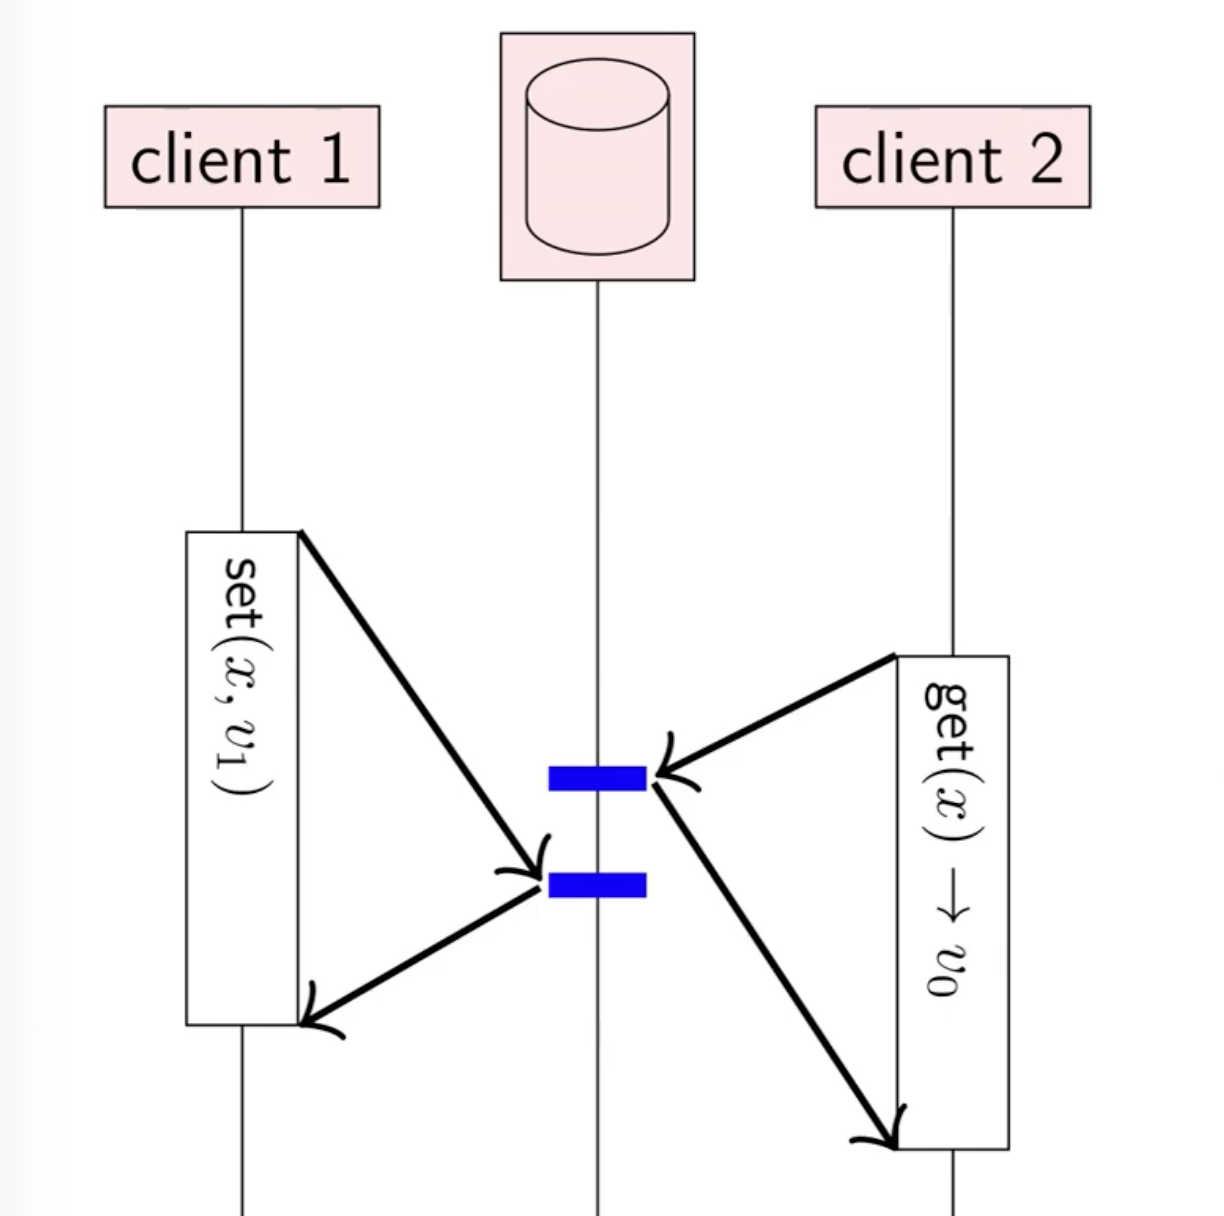
\includegraphics[scale=0.25]{computer-sceince/distributed-media/linearization.png}
        \caption{ If both overlap in time, it is okay that one starts after the other or the other way around
        }
\end{figure}

Some distributed systems do not provide linearization. 
for instance, quorum write, but not quorum read (quorum is performed only by the client).

\begin{figure}[t]
    \centering
    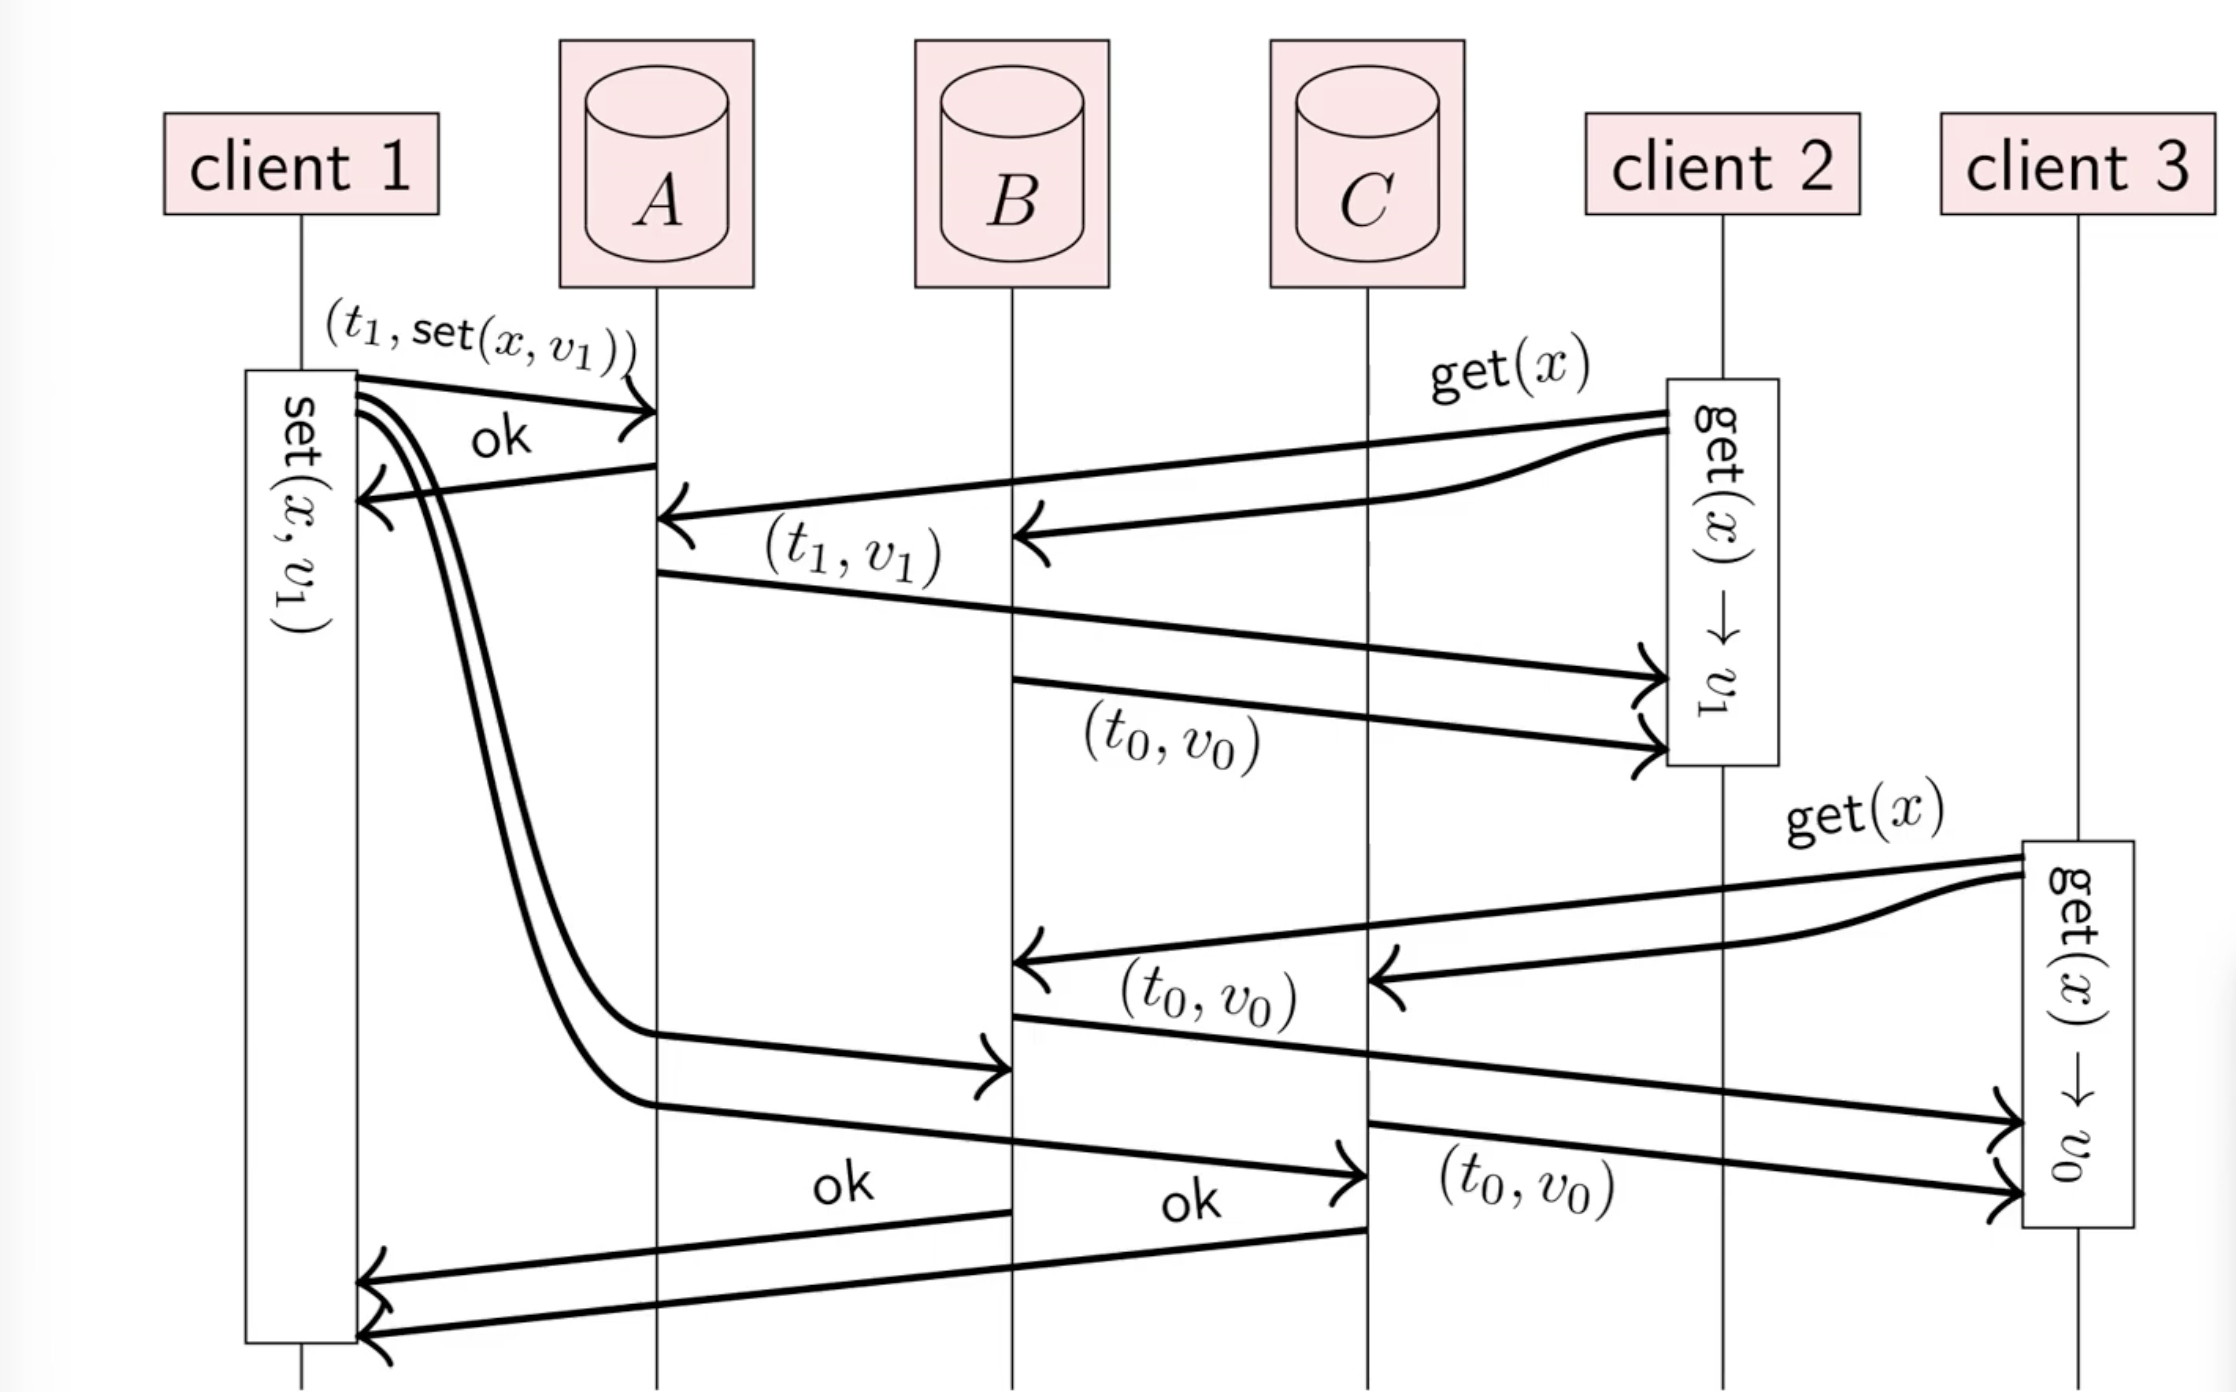
\includegraphics[scale=0.25]{computer-sceince/distributed-media/linearization-failure.png}
    \caption{Notice that $client_3$ started after $client_2$, but got value
    from version $v_0$, while $client_2$ got the value from version $v_1$.
    }
\end{figure}

\todo{could not find formal definition.}

